\section{Aufbau}

Der Versuchsaufbau ist in Abbildung \ref{fig:aufb} dargestellt. Zunächst wird um eine Cd-Lampe ein 
Elektromagnet aufgebaut, da ohne Magnetfeld kein Zeeman-Effekt zu sehen wäre.
Dann wird senkrecht zum Magnetfeld das Licht kollimiert und durch ein Gradsichtprisma in seine verschiedenen 
Wellenlängen aufgeteilt. Anschließend wird ein Polarisationsfilter und ein Spalt angebracht, sodass das 
gewollte Licht herausgefiltert werden kann. 

\begin{figure}
  \centering
  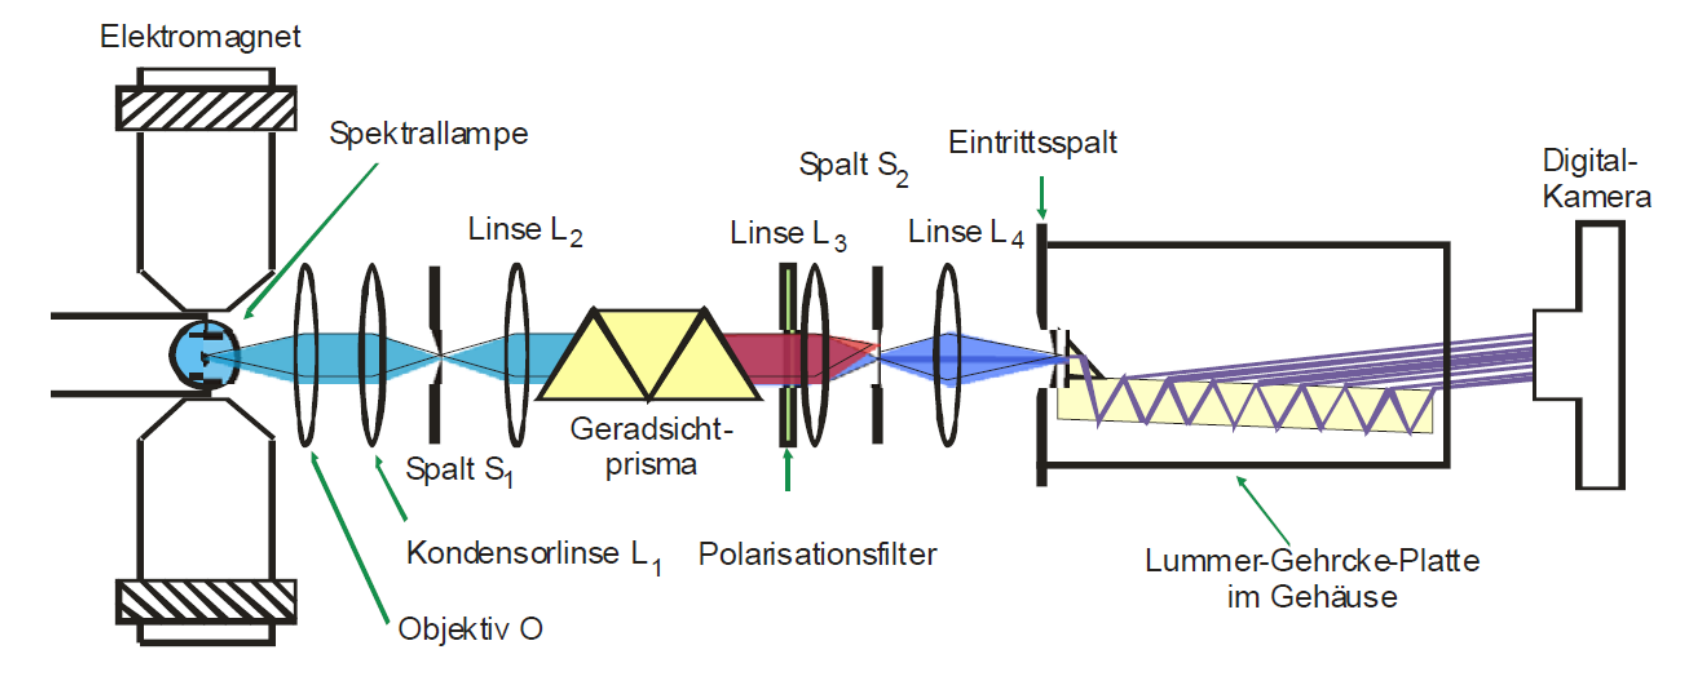
\includegraphics[width=0.75\textwidth]{aufbau.png}
  \caption{Versuchsaufbau[1].}
  \label{fig:aufb}
\end{figure}
\FloatBarrier

Zum Schluss wird das ausgewählte Licht auf eine Lummer-Gehrcke-Platte geleitet, diese teilt den Lichtstrahl 
in mehrere parallele Lichtbündel die miteinander interferieren. 
Sie ist in Abblildung \ref{fig:pl} dargestellt. 

\begin{figure}
  \centering
  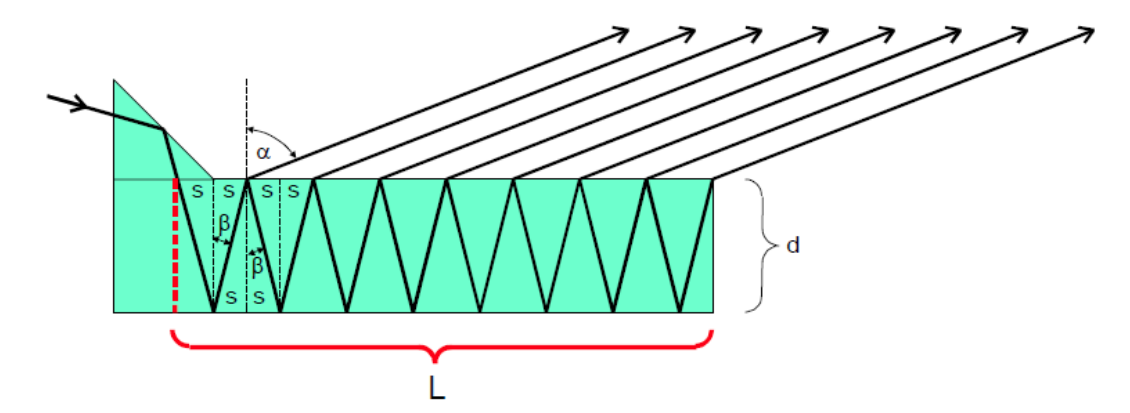
\includegraphics[width=0.75\textwidth]{platte.png}
  \caption{Lummer-Gehrcke-Platte[1].}
  \label{fig:pl}
\end{figure}
\FloatBarrier

Bei monochromatischem Licht ist die Bedingung für konstruktive Interferenz abhängig von der Wellenlänge und 
der Dicke der Platte $d$. Es entstehen Interferenzstreifen mit einem Gangunterschied von $\lambda$. 
Der Gangunterschied entspricht also der Wellenlänge des eingestrahlten Lichtes. Der Gangunterschied ändert sich durch  
einschalten des Magnetfeldes um die Aufspaltung 
\begin{equation}
  \delta \lambda = \frac{1}{2} \frac{\delta s}{\symup{\Delta}s} \symup{\Delta}\lambda_{\si{D}}.
  \label{dl}
\end{equation}
Mithilfe der Formel 
\begin{equation}
  g = \frac{h c \delta \lambda}{\lambda² \mu_B B},
  \label{eqn:g}
\end{equation}
können daraus auch die Landé-Faktoren bestimmt werden.

Die Messung kann bei einem großen Austrittswinkel nur innerhalb des Dispersionsgebiets
\begin{equation}
  \symup{\Delta}\lambda_{\si{D}} = \frac{\lambda²}{2 d} \sqrt{\frac{1}{n²-1}}
  \label{eqn:lD}
\end{equation}
stattfinden, wobei $n$ der Brechungsindex ist. Das Dispersionsgebiet ist dabei die Differenz, die zwei Wellenlängen 
maximal haben dürfen, damit sie sich nicht überlagern.
Das Auflösungsvermögen $A$ berechnet sich dann durch
\begin{equation}
  A = \frac{\lambda}{\symup{\Delta}\lambda_{\si{D}}} = \frac{L}{\lambda} (n²-1),
  \label{eqn:A}
\end{equation} 
wobei $L$ die Länge der Platte ist. 



\section{Durchführung}
\label{sec:Durchführung}

Zunächst muss das Magnetfeld des Elektromagneten geeicht werden, d.h. den einstellbaren Stomstärken des 
Elektromagneten soll eine konkrete Feldstärke zugeorndet werden. Dafür werden die einstellbaren Stromstärken
durchlaufen, und zu den Stomstärke-Werten die passenden Magnetfelder mit einer Hall-Sonde in der Nähe der 
Cd-Lampe ausgemessen und als Wertepaare aufgenommen. 

Nun wird die rote Linie durch den Spalt ausgewählt, dann wird der Polarisationsfilter auf Null gestellt, 
sodass die $\pi$-Übergänge zu sehen sind.
Dann muss der Aufbau so eingestellt werden, dass nach durchlaufen der Lummer-Gehrcke-Platte ein Interferenzbild 
zu sehen ist. Dafür müssen die Linsen richtig positioniert sein. %und erst ohne platte scharf zu sehen. dann mit platte und auge gut zu sehen
Anschließend wird das Bild mit einer Kamera aufgenommen. Da die Intensiät des Lichtes auf der Lummer-Gehrcke-Platte 
sehr gering ist, müssen dafür alle anderen Lichtquellen abgedunkelt werden. 
Zum Schluss wird der Polarisationsfilter nochmal auf $\frac{\lambda}{4}$ gestellt, 
sodass nun die $\sigma$-Übergänge analog aufgenommen werden können. 

Der Ablauf wird für die blaue Spekrallinie wiederholt.

Das Magnetfeld wird dabei opimal eingestellt, gemäß Teil \ref{sec:bo}.